\documentclass{article}
\usepackage[utf8]{inputenc}
\usepackage[margin=1in]{geometry}
\usepackage{graphicx}
\usepackage{listings}
\usepackage{xcolor}
\usepackage{hyperref}
\usepackage{tikz}
\usetikzlibrary{calc}
\usetikzlibrary{positioning, arrows.meta}
\usetikzlibrary{shapes.geometric, arrows, positioning}

% Fix for duplicate page identifier warning
\hypersetup{hypertexnames=false}

% Simple code styling
\lstset{
    basicstyle=\ttfamily\small,
    breaklines=true,
    commentstyle=\color{green!40!black},
    keywordstyle=\color{blue},
    frame=single,
    captionpos=b,
    language=Python
}

\title{Technical Documentation: ANE2 Remote RF Sensor System}
\author{Engineering Team}
\date{\today}

\begin{document}

\maketitle
\tableofcontents
\newpage

\section{System Overview}
The ANE2 system is a remote RF sensor platform designed for high-performance data acquisition, signal processing, and scheduled measurement campaigns. It utilizes a Raspberry Pi as the core compute node to manage specialized hardware like the HackRF.

\section{Software Architecture}
The software is organized into a modular daemon-based architecture to ensure reliability.

\subsection{System Daemons}
The system is managed by several \texttt{systemd} units generated during the provisioning phase:
\begin{itemize}
    \item \textbf{rf-ane2.service}: Core RF application for data acquisition.
    \item \textbf{orchestrator-ane2.service}: Central engine for state management.
    \item \textbf{status-ane2.service/timer}: Periodic health monitoring.
    \item \textbf{ltegps-ane2.service}: Telemetry and location data.
\end{itemize}

\section{The Orchestrator \& System Logic}

The \texttt{orchestrator.py} module serves as the central cognitive unit of the ANE2 system. It is responsible for high-level decision-making, state transition management, and ensuring that hardware resources are utilized efficiently without task overlap.

\subsection{Global State Machine}
The system's behavior is governed by a formal state machine defined in the \texttt{SysState} enumeration. Transitions are managed by the \texttt{GlobalSys} controller, which enforces mutual exclusivity between tasks.

\begin{itemize}
    \item \textbf{IDLE}: The default resting state. The system polls the API for new real-time instructions or scheduled measurement windows.
    \item \textbf{REALTIME}: Triggered by user demand via the API. In this state, the system provides a continuous stream of spectral data and optional demodulated audio.
    \item \textbf{CAMPAIGN}: Activated when a scheduled measurement window opens. The system executes high-priority tasks defined by the central server.
    \item \textbf{KALIBRATING}: A transient state where the system runs \texttt{kal\_sync.py} to correct clock drift and frequency offsets before starting a campaign.
    \item \textbf{ERROR}: A safety state entered upon critical hardware or network failure.
\end{itemize}



\subsection{Real-time Operational Loop}
When in \texttt{REALTIME} mode, the orchestrator enters a "Sticky" execution loop. It performs a continuous heartbeat with the API to fetch \texttt{ServerRealtimeConfig} objects.

\begin{itemize}
    \item \textbf{WebRTC Integration}: If demodulation (AM/FM) is requested, the orchestrator spawns a \texttt{server\_webrtc.py} subprocess to handle low-latency audio distribution.
    \item \textbf{Dynamic Configuration}: The loop monitors changes in center frequency, sample rate, and gains. If a demodulation change is detected, it sends a synchronization command to the RF Engine via ZMQ to reset the DSP pipeline.
\end{itemize}

\subsection{Campaign Management and Crontab Synchronization}
The \texttt{CronSchedulerCampaign} class manages the persistence of measurement tasks. Unlike real-time tasks, campaigns are scheduled at the OS level to ensure reliability.

\begin{itemize}
    \item \textbf{Priority Logic}: If multiple campaigns overlap in the same time window, the scheduler applies a "Winner-Takes-All" strategy, selecting the campaign with the highest \texttt{campaign\_id}.
    \item \textbf{System Integration}: Valid campaigns are converted into standard Linux \texttt{cron} entries with the comment prefix \texttt{CAMPAIGN\_[ID]}.
    \item \textbf{State Persistence}: Campaign parameters are stored in the \texttt{ShmStore} (Shared Memory), allowing the \texttt{campaign\_runner.py} to access hardware settings even after a system reboot.
\end{itemize}

\subsection{Advanced Acquisition Strategies (AcquireDual)}
To mitigate artifacts inherent in low-cost SDR hardware, the orchestrator utilizes the \texttt{AcquireDual} engine. This component implements two primary correction strategies:

\subsubsection{DC Spike Removal}
The "Center Spike" artifact is removed by sampling the noise floor in the immediate vicinity of the center frequency. The engine then injects synthetic Gaussian noise into the central 0.2\% of the bins, matching the local mean and standard deviation ($\mu, \sigma$) to maintain spectral integrity.

\subsubsection{Spectral Stitching (Cosido)}
For high-precision captures, the system performs a dual-acquisition "Stitching" technique:
\begin{enumerate}
    \item Capture A is taken at the desired center frequency ($f_c$).
    \item Capture B is taken with a frequency offset (e.g., $+2$ MHz).
    \item A linear correction ramp is calculated to align the amplitudes of both captures.
    \item A cosine-faded blending mask is applied to merge the clean data from Capture B into the distorted center of Capture A.
\end{enumerate}

\begin{center}
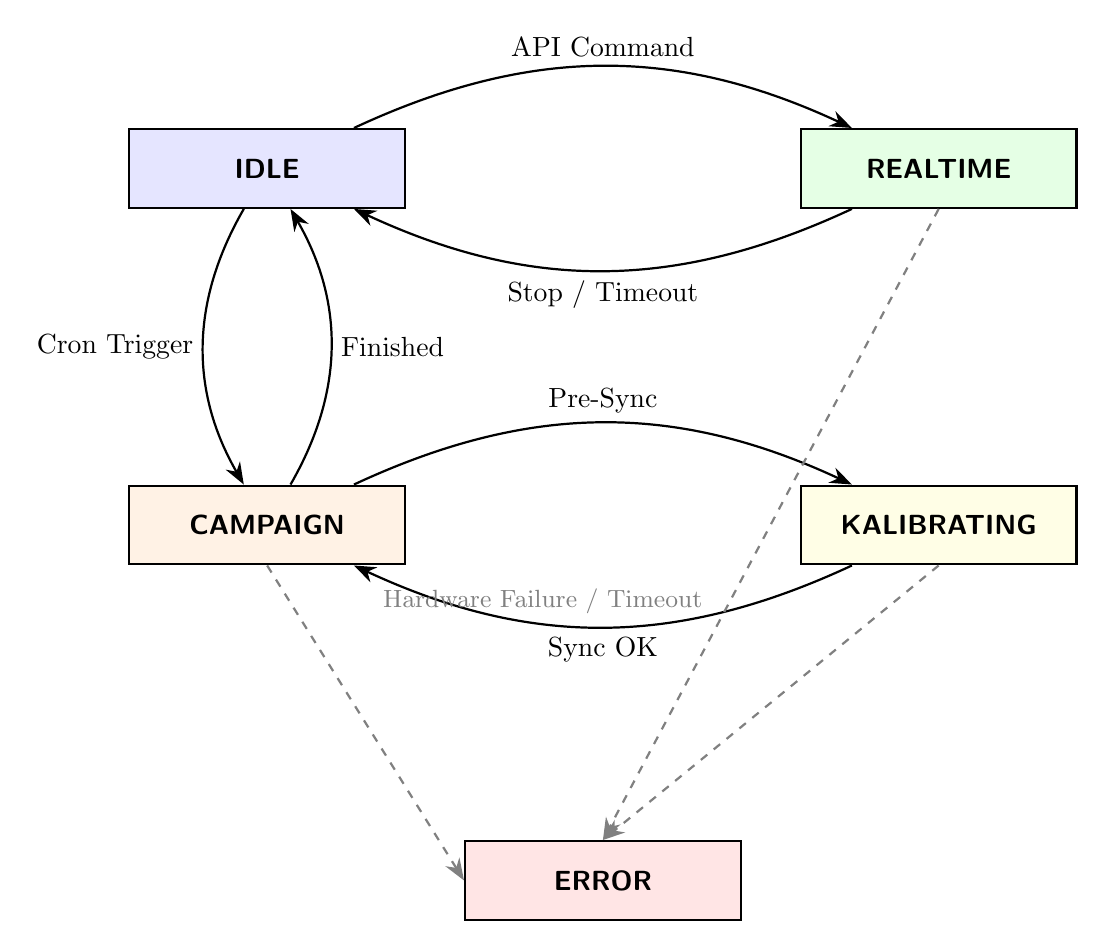
\begin{tikzpicture}[
    node distance=3.5cm and 5cm, 
    auto, 
    thick,
    state/.style={rectangle, draw, minimum width=3.5cm, minimum height=1cm, font=\sffamily\bfseries},
    arrow/.style={-{Stealth[scale=1.2]}}
]
    % State nodes
    \node (idle) [state, fill=blue!10] {IDLE};
    \node (real) [state, fill=green!10, right=of idle] {REALTIME};
    \node (camp) [state, fill=orange!10, below=of idle] {CAMPAIGN};
    \node (kal)  [state, fill=yellow!10, right=of camp] {KALIBRATING};
    
    % Error node positioned at the bottom to avoid overlapping loops
    \node (err)  [state, fill=red!10, below=of $(camp)!0.5!(kal)$, yshift=-0.5cm] {ERROR};

    % Transitions: IDLE <-> REALTIME
    \path [arrow] (idle) edge [bend left=25] node [above] {API Command} (real);
    \path [arrow] (real) edge [bend left=25] node [below] {Stop / Timeout} (idle);

    % Transitions: IDLE <-> CAMPAIGN
    % Cron goes DOWN to start; Finished goes UP to end
    \path [arrow] (idle) edge [bend right=30] node [left] {Cron Trigger} (camp);
    \path [arrow] (camp) edge [bend right=30] node [right] {Finished} (idle);

    % Transitions: CAMPAIGN <-> KALIBRATING
    \path [arrow] (camp) edge [bend left=25] node [above] {Pre-Sync} (kal);
    \path [arrow] (kal)  edge [bend left=25] node [below] {Sync OK} (camp);

    % Universal Error Transitions (Dashed to indicate interrupt)
    \draw [arrow, dashed, gray] (real.south) -- (err.north);
    \draw [arrow, dashed, gray] (kal.south) -- (err.north);
    \draw [arrow, dashed, gray] (camp.south) -- (err.west);
    
    % Optional: Label for error transitions
    \node [gray, font=\small] at (3.5, -5.5) {Hardware Failure / Timeout};

\end{tikzpicture}
\end{center}

\section{System Monitoring and Status}
The \texttt{status.py} module implements the \texttt{StatusDevice} class, which performs low-overhead hardware monitoring by reading directly from the Linux virtual filesystems (\texttt{/proc} and \texttt{/sys}). It captures:
\begin{itemize}
    \item CPU usage per core from \texttt{/proc/stat}.
    \item RAM and Swap utilization from \texttt{/proc/meminfo}.
    \item SoC temperature from \texttt{thermal\_zone0}.
    \item Network latency via ICMP pings.
\end{itemize}

\section{System Initialization}
The \texttt{init\_sys.py} script provisions the environment, creates directories (\texttt{Logs}, \texttt{Queue}), and resets shared memory.


\end{document}